%\documentclass{beamer}
\documentclass[handout]{beamer}
%\documentclass{beamer}
%\usepackage{xeCJK}
\usepackage{ctex}

\usepackage[orientation=landscape,size=custom,width=16,height=12,scale=0.5,debug]{beamerposter}

 % 1. packages

 % ----------- fonts and symbles ---------
\usepackage{amsmath,amssymb,amsfonts,amsthm}
%\usepackage{CJK}
\usepackage{dsfont}
\usepackage{mathrsfs}
\usepackage{eucal} % for \mathcal

%\renewcommand{\rmdefault}{ptm}


%\usepackage{fontspec}
%\newfontfamily\monaco{Monaco}

%\usepackage{mathbbold} %,bbold

 \usepackage{textcomp} % for \textnormal{\textperthousand}
% -----------------





%\usepackage{slashbox}
%\usepackage[margin=2.2cm]{geometry} % |geometry| package clash with |booktabs| package
%\usepackage{cases}
% -------- tables -------
\usepackage{booktabs} % for \toprule, \bottomrule
\usepackage{tabularx}
\usepackage{multirow}
% --------- figures ---------
\usepackage{graphicx}
% ---------- algorithms -------
\usepackage{algorithm}
\usepackage{algorithmic}
%\usepackage{footnote}
    % |footnote| package occurs error:
    % Runaway argument?
    % \def \insertfootnotetext {\@@ }\def \insertfootnotemark {\@makefnmark \ETC.

\usepackage{listings}

\usepackage[linewidth=1pt]{mdframed} % for  mdframe environment




 \usepackage{color}
 \usepackage{xcolor}     %¸ßÁÁʹÓõÄÑÕÉ«

\usepackage{setspace}
%%\usepackage{type1cm}
\usepackage{adjustbox} % for \adjustbox

\usepackage{accsupp}
\newcommand{\emptyaccsupp}[1]{\BeginAccSupp{ActualText={}}#1\EndAccSupp{}}




%%   figures and tables
\graphicspath{{figure/}}


% 2. new commands

% 2.0 common commands
%\newcommand{\bc}{\begin{center}}
%\newcommand{\ec}{\end{center}}
%\newcommand{\ba}{\begin{array}}
%\newcommand{\ea}{\end{array}}
%\newcommand{\be}{\begin{equation}}
%\newcommand{\ee}{\end{equation}}

% 2.1 colors
\definecolor{dgrey}{rgb}{0.30,0.30,0.30}
\definecolor{lred}{rgb}{0.50,0.00,0.50}
\definecolor{lblue}{rgb}{0.8,0.8,1}
\definecolor{dred}{rgb}{0.6,0,0}
\definecolor{dblue}{rgb}{0,0,0.5}
\definecolor{dgrey}{rgb}{0.35,0.35,0.35}
\definecolor{rred}{rgb}{0.9,0,0}
\definecolor{mylblue}{rgb}{0.3,0.2, 0.8}

\definecolor{commentcolor}{RGB}{85,139,78}
\definecolor{stringcolor}{RGB}{206,145,108}
\definecolor{keywordcolor}{RGB}{34,34,250}
\definecolor{backcolor}{RGB}{220,220,220}

\newcommand{\blue}[1]{{\color{blue}#1}}
\newcommand{\dblue}[1]{{\color{dblue}#1} }
\newcommand{\red}[1]{{\color{red}#1}}
\newcommand{\dred}[1]{{\color{dred}#1}}
\newcommand{\cyan}[1]{{\color{cyan}#1}}
\newcommand{\bfblue}[1]{\textbf{\color{dblue}#1} }
\newcommand{\bfred}[1]{\textbf{\color{dred}#1} }
\newcommand{\green}[1]{{\color{green}#1}}
%\newcommand{\alert}[1]{{\color{red}#1}}
\newcommand{\black}[1]{{\color{black}#1}}
\newcommand{\light}[1]{{\color{blue}\textbf{#1}}}
\newcommand{\hot}[1]{{\color{dred}#1}}
 \newcommand{\highlight}[1]{ \textbf{\color{mylblue}#1}}
 \newcommand{\important}[1]{{\color{red}#1}} % for highlighting  some words

 \newcommand{\mystar}{\dred{$^{\clubsuit}$ }}
  \newcommand{\doublestar}{\dred{$^{\clubsuit\clubsuit}$ }}

\newcommand{\mynote}[1]{{\footnotesize \color{mylblue}#1}}

 \newcommand{\hint}[1]{{\small \color{mylblue}#1}}
\newcommand{\smallhint}[1]{{\small \color{dgrey}#1}}
\newcommand{\footnotehint}[1]{{\footnotesize \color{dgrey}#1}}
\newcommand{\tinyhint}[1]{{\tiny \color{dgrey}#1}}
\newcommand{\mytitle}[1]{\medskip{\large \textbf{\color{mylblue}#1}}}
\newcommand{\normaltitle}[1]{\medskip{ \textbf{\color{mylblue}#1}}}

%\newcommand{\head}[1]{\textbf{\large\color{blue}#1}}
%\newcommand{\heading}[1]{\textbf{\large\color{blue}#1}}

\newcommand{\myfbox}[2]{ \bigskip \begin{center} \fbox{\parbox{#1}{ #2  }} \end{center}\bigskip }

\newcommand{\myvar}[1]{}
%\newcommand{\mynote}[1]{#1}

% 2.2 mathematical symbols

\newcommand{\drightarrow}{\stackrel{d.}{\rightarrow}}
\newcommand{\prightarrow}{\stackrel{p.}{\rightarrow}}
\newcommand{\bernoulli}{\textnormal{Ber}}
\newcommand{\cov}{\mathsf{Cov}}
\newcommand{\corr}{\mathbf{Corr}}
\newcommand{\regret}{\textnormal{Regret}}
\newcommand{\conv}{\textnormal{conv}}
\newcommand{\dotdiv}{\stackrel{\centerdot}{-}}
\newcommand{\dom}{\textnormal{dom}}
\newcommand{\convergenceinprob}{\stackrel{P}{\rightarrow}}
\newcommand{\convergenceindist}{\rightsquigarrow}
\newcommand{\probability}{\mathbb{P}}
\newcommand{\expectation}{\mathbb{E}}
\newcommand{\epi}{\textnormal{epi}}
\newcommand{\variance}{\mathbb{V}}
\newcommand{\var}[1]{\mathbb{V}(#1)}
\newcommand{\covariance}{\mathsf{Cov}}
\newcommand{\empiricalrisk}[1]{\hat{R}(#1)}
\newcommand{\expectedrisk}[1]{R(#1)}
\newcommand{\mgf}[1]{\psi_{#1}(\lambda)}
\newcommand{\mgfexpansion}[1]{\expectation[e^{\lambda#1}]}
\newcommand{\mgfmultivariate}[1]{\expectation[e^{\lambda^\transpose#1}]}
\newcommand{\transpose}{{\mathsf{T}}}
\newcommand{\real}{\mathbb{R}}
\newcommand{\gaussian}[2]{\mathcal{N}(#1,#2)}
\newcommand{\subGaussian}[1]{\mathsf{subG}(#1)}
\newcommand{\indicator}[1]{\mathbb{I}[#1]}
\newcommand{\x}[1]{x^{(#1)}}
\newcommand{\y}[1]{y^{(#1)}}
\newcommand{\z}[1]{z^{(#1)}}
\newcommand{\feature}{x}
\newcommand{\response}{y}
\newcommand{\supofempiricalprocess}{\|\mathbb{P}_n-\mathbb{P}\|_{\decisionspace}}
\newcommand{\decisionspace}{\mathscr{F}}
\newcommand{\decisionfunction}{f}
\newcommand{\featurespace}{\mathcal{X}}
\newcommand{\classifierestimate}{\widehat{h}}
\newcommand{\classifiertrue}{h^\star}
\newcommand{\classifier}{h}
\newcommand{\hypothesisclass}{\mathcal{H}}
\newcommand{\dataset}{\mathcal{D}}
\newcommand{\defineas}{\stackrel{\textnormal{def}}{=}}
\newcommand{\rademachercomplexity}[1]{\mathsf{Rad}_n\left(#1\right)}
\newcommand{\loss}{\ell}
\newcommand{\composite}{\circ}
\newcommand{\convexhull}{\mathsf{conv}}
\newcommand{\norm}[2][2]{\|#2\|_{#1}}
\newcommand{\shatteringcoefficient}[2]{\mathcal{S}(#1,#2)}
\newcommand{\vcdimension}[1]{\mathsf{VC}\left(#1\right)}
\newcommand{\rank}{\mathsf{rank}}
\newcommand{\innerproduct}[2]{\left\langle #1, #2\right\rangle}
\newcommand{\modelparameter}{\theta}
\newcommand{\ball}[3][]{\mathcal{B}_{{#1}}\left(#2,#3\right)}
\newcommand{\metric}{d}
\newcommand{\coveringnumber}[4][]{N_{{#1}}\left(#2,#3,#4\right)}
\newcommand{\trace}{\textnormal{tr}}
\newcommand{\std}{\textnormal{std}}
\newcommand{\sgn}{\textnormal{sign}}
%\renewcommand{\span}{\textnormal{span}}

 % do not overwrite the existing command \span
 % as it leads to an error of
 %  "Missing # Inserted in Alignment Preamble" for ``align'' environment

\newcommand{\myspan}{\textnormal{span}}

%%%
\newcommand{\rightarrowd}{\stackrel{d}{\rightarrow}}
\newcommand{\rightarrowp}{\stackrel{p}{\rightarrow}}
\newcommand{\defeq}{ \stackrel{\textnormal{def}}{=}}
\newcommand{\proj}{ \textnormal{Proj}}
\newcommand{\dist}{\textnormal{dist}}

\newcommand{\argmax}{\textnormal{argmax}}
\newcommand{\argmin}{\textnormal{argmin}}
\newcommand{\subg}{\textnormal{subG}}


 \newcommand{\bba}{\mathbb{A}}
\newcommand{\bbb}{\mathbb{B}}
\newcommand{\bbc}{\mathbb{C}}
\newcommand{\bbd}{\mathbb{D}}
\newcommand{\bbe}{\mathbb{E}}
\newcommand{\bbf}{\mathbb{F}}
\newcommand{\bbg}{\mathbb{G}}
\newcommand{\bbh}{\mathbb{H}}
\newcommand{\bbi}{\mathbb{I}}
\newcommand{\bbj}{\mathbb{J}}
\newcommand{\bbk}{\mathbb{K}}
\newcommand{\bbl}{\mathbb{L}}
\newcommand{\bbm}{\mathbb{M}}
\newcommand{\bbn}{\mathbb{N}}
\newcommand{\bbo}{\mathbb{O}}
\newcommand{\bbp}{\mathbb{P}}
\newcommand{\bbq}{\mathbb{Q}}
\newcommand{\bbr}{\mathbb{R}}
\newcommand{\bbs}{\mathbb{S}}
\newcommand{\bbt}{\mathbb{T}}
\newcommand{\bbu}{\mathbb{U}}
\newcommand{\bbv}{\mathbb{V}}
\newcommand{\bbw}{\mathbb{W}}
\newcommand{\bbx}{\mathbb{X}}
\newcommand{\bby}{\mathbb{Y}}
\newcommand{\bbz}{\mathbb{Z}}

\newcommand{\bfa}{\mathbf{a}}
\newcommand{\bfb}{\mathbf{b}}
\newcommand{\bfc}{\mathbf{c}}
\newcommand{\bfd}{\mathbf{d}}
\newcommand{\bfe}{\mathbf{e}}
\newcommand{\bff}{\mathbf{f}}
\newcommand{\bfg}{\mathbf{g}}
\newcommand{\bfh}{\mathbf{h}}
\newcommand{\bfi}{\mathbf{i}}
\newcommand{\bfj}{\mathbf{j}}
\newcommand{\bfk}{\mathbf{k}}
\newcommand{\bfl}{\mathbf{l}}
\newcommand{\bfm}{\mathbf{m}}
\newcommand{\bfn}{\mathbf{n}}
\newcommand{\bfo}{\mathbf{o}}
\newcommand{\bfp}{\mathbf{p}}
\newcommand{\bfq}{\mathbf{q}}
\newcommand{\bfr}{\mathbf{r}}
\newcommand{\bfs}{\mathbf{s}}
\newcommand{\bft}{\mathbf{t}}
\newcommand{\bfu}{\mathbf{u}}
\newcommand{\bfv}{\mathbf{v}}
\newcommand{\bfw}{\mathbf{w}}
\newcommand{\bfx}{\mathbf{x}}
\newcommand{\bfy}{\mathbf{y}}
\newcommand{\bfz}{\mathbf{z}}

\newcommand{\bfA}{\mathbf{A}}
\newcommand{\bfB}{\mathbf{B}}
\newcommand{\bfC}{\mathbf{C}}
\newcommand{\bfD}{\mathbf{D}}
\newcommand{\bfE}{\mathbf{E}}
\newcommand{\bfF}{\mathbf{F}}
\newcommand{\bfG}{\mathbf{G}}
\newcommand{\bfH}{\mathbf{H}}
\newcommand{\bfI}{\mathbf{I}}
\newcommand{\bfJ}{\mathbf{J}}
\newcommand{\bfK}{\mathbf{K}}
\newcommand{\bfL}{\mathbf{L}}
\newcommand{\bfM}{\mathbf{M}}
\newcommand{\bfN}{\mathbf{N}}
\newcommand{\bfO}{\mathbf{O}}
\newcommand{\bfP}{\mathbf{P}}
\newcommand{\bfQ}{\mathbf{Q}}
\newcommand{\bfR}{\mathbf{R}}
\newcommand{\bfS}{\mathbf{S}}
\newcommand{\bfT}{\mathbf{T}}
\newcommand{\bfU}{\mathbf{U}}
\newcommand{\bfV}{\mathbf{V}}
\newcommand{\bfW}{\mathbf{W}}
\newcommand{\bfX}{\mathbf{X}}
\newcommand{\bfY}{\mathbf{Y}}
\newcommand{\bfZ}{\mathbf{Z}}


\newcommand{\bfSigma}{\mathbf{\Sigma}}
\newcommand{\bfrho}{\mathbf{\rho}}

\newcommand{\cala}{\mathcal{A}}
\newcommand{\calb}{\mathcal{B}}
\newcommand{\calc}{\mathcal{C}}
\newcommand{\cald}{\mathcal{D}}
\newcommand{\cale}{\mathcal{E}}
\newcommand{\calf}{\mathcal{F}}
\newcommand{\calg}{\mathcal{G}}
\newcommand{\calh}{\mathcal{H}}
\newcommand{\cali}{\mathcal{I}}
\newcommand{\calj}{\mathcal{J}}
\newcommand{\calk}{\mathcal{K}}
\newcommand{\call}{\mathcal{L}}
\newcommand{\calm}{\mathcal{M}}
\newcommand{\caln}{\mathcal{N}}
\newcommand{\calo}{\mathcal{O}}
\newcommand{\calp}{\mathcal{P}}
\newcommand{\calq}{\mathcal{Q}}
\newcommand{\calr}{\mathcal{R}}
\newcommand{\cals}{\mathcal{S}}
\newcommand{\calt}{\mathcal{T}}
\newcommand{\calu}{\mathcal{U}}
\newcommand{\calv}{\mathcal{V}}
\newcommand{\calw}{\mathcal{W}}
\newcommand{\calx}{\mathcal{X}}
\newcommand{\caly}{\mathcal{Y}}
\newcommand{\calz}{\mathcal{Z}}


% 3. theorem and environments

%\newtheorem{theorem}{Theorem}%[section]
\newtheorem{proposition}{Proposition}%[section]
%\newtheorem{property}{Property}%[section]
%\newtheorem{lemma}{Lemma}%[section]
%\newtheorem{corollary}{Corollary}%[section]
%\newtheorem{definition}{Definition}%[section]
%\newtheorem{example}{Example}%[section]
%\newtheorem{remark}{Remark}%[section]
%\newtheorem{note}{Note}%[section]
%\newtheorem{problem}{Problem}%[section]
\newtheorem{exercise}{Exercise}
%\newtheorem{assumption}{Assumption}
\newtheorem*{lemma_star}{Lemma}
\newtheorem*{theorem_star}{Theorem}

%\newenvironment{summary}[1][Summary]{\par\medskip   \color{dred}\textbf{\large#1. } }{ \medskip}
%\newenvironment{remark}[1][Remark]{\par\medskip  \begin{small} \color{dblue}\textbf{#1. } }{ \end{small}\medskip}
%\renewenvironment{proof}[1][Proof]{\noindent\textbf{#1.} }{\mbox{} \hfill{\small\textrm{$\Box$}}\vspace{1ex}}
% \newenvironment{answer}[1][Answer]{\par\medskip \color{dblue}\textbf{\large#1. }}{ \medskip}

\newenvironment{summary}[1][总结]{\par\medskip   \color{dred}\textbf{\large#1 } }{ \medskip}
\newenvironment{remark}[1][注意]{\par\medskip   \color{dblue}\textbf{\large#1 } }{ \medskip}
\newenvironment{footnoteremark}{ \color{dblue}\begin{footnotesize} }{\end{footnotesize}}
\renewenvironment{proof}[1][证明]{\noindent\textbf{#1.} }{\mbox{} \hfill{\small\textrm{$\Box$}}\vspace{1ex}}
 \newenvironment{question}[1][Q.]{\par\medskip {\color{lred}\large#1}}{ \medskip}
 \newenvironment{answer}[1][Answer]{\par\medskip \color{dblue}\textbf{\large#1 }}{ \medskip}

% 4. beamer setting




%\newtheorem{definition}{\textbf{¶¨Òå}}[section]
%\newtheorem{proposition}[definition] { \textbf{ÃüÌâ}}
%\newtheorem{lemma}[definition] { \textbf{ÒýÀí}}
%\newtheorem{theorem}[definition]{ \textbf{¶¨Àí}}
%\newtheorem{corollary}[definition] { \textbf{ÍÆÂÛ}}
%\newtheorem{remark}[definition] { \textbf{×¢}}
%\newtheorem{example}[definition] { \textbf{Àý}}

%\newcommand{\shadow}[1]{\begin{center}
%\bf{\textcolor{dblue}{\shadowbox{\parbox{3.8in}
% {\textcolor{red}
% {\vspace{1mm}#1}}}}}
%\end{center}}
%
%\newcommand{\head}[1]{\begin{center}
%\bf{\textcolor{dblue}{\shadowbox{\parbox{3.8in}
% {\textcolor{dred}
% {\vspace{1mm}#1}}}}}
%\end{center}}
%
%
%\newcommand{\heading}[1]{%
%  \begin{center}
%    \large\bf
%    \shadowbox{#1}%
%  \end{center}
%\vspace{1ex minus 1ex}}

% set  space above and below math equations in display style

\expandafter\def\expandafter\normalsize\expandafter{%
    \normalsize
    \setlength\abovedisplayskip{1.5ex}
    \setlength\belowdisplayskip{1.2ex}
    \setlength\abovedisplayshortskip{0.5ex}
    \setlength\belowdisplayshortskip{0.5ex}
}

% Ìí¼ÓÒ³Âë´úÂ룬¹È¸èÕÒµ½µÄ¡£
\addtobeamertemplate{navigation symbols}{}{%
    %\usebeamerfont{footline}%
    %\usebeamercolor[fg]{footline}%
    \setbeamercolor{footline}{fg=blue}
    \setbeamerfont{footline}{series=\bfseries}
    \hspace{1em}%
    \normalsize{\insertframenumber/\inserttotalframenumber}
}

% section numbering
\setbeamertemplate{section in toc}[sections numbered]
\setbeamertemplate{subsection in toc}[subsections numbered]



\lstset{                        %¸ßÁÁ´úÂëÉèÖÃ
%basicstyle=\small, % print whole listing small
%basicstyle=\footnotesize\sffamily, % print whole listing small
basicstyle=\footnotesize\rmfamily, % print whole listing small
%basicstyle=\rmfamily, % print whole listing small
    language=python,                    %PythonÓï·¨¸ßÁÁ
    %linewidth=0.9\linewidth,            %Áбílist¿í¶È
    %basicstyle=\ttfamily,              %ttÎÞ·¨ÏÔʾ¿Õ¸ñ
    commentstyle=\color{commentcolor},  %×¢ÊÍÑÕÉ«
    keywordstyle=\color{keywordcolor},  %¹Ø¼ü´ÊÑÕÉ«
    stringstyle=\color{stringcolor},    %×Ö·û´®ÑÕÉ«
    %showspaces=true,                   %ÏÔʾ¿Õ¸ñ
    numbers=left,                       %ÐÐÊýÏÔʾÔÚ×ó²à
    %numberstyle=\tiny\emptyaccsupp,     %ÐÐÊýÊý×Ö¸ñʽ
    numberstyle=\tiny,                  %ÐÐÊýÊý×Ö¸ñʽ
    numbersep=5pt,                      %Êý×Ö¼ä¸ô
    frame=single,                       %¼Ó¿ò
    framerule=0pt,                      %²»»®Ïß
    %escapeinside=@@,                    %ÌÓÒݱêÖ¾
    escapeinside=``,                    %ÌÓÒݱêÖ¾
    emptylines=1,                       %
    xleftmargin=3em,                    %list×ó±ß¾à
    backgroundcolor=\color{backcolor},  %ÁÐ±í±³¾°É«
    tabsize=4,                          %ÖƱí·û³¤¶ÈΪ4¸ö×Ö·û
    %gobble=4                            %ºöÂÔÿÐдúÂëÇ°4¸ö×Ö·û
    breaklines=true,
    extendedchars=false
    }

\lstdefinestyle{numbers}{numbers=left, stepnumber=1, numberstyle=\tiny, numbersep=10pt}
 \lstdefinestyle{nonumbers}{numbers=none}

\newcommand{\alertcode}[1]{{\color{red}#1}} % used for alerting codes

%\lstset{numbers=left, numberstyle=\tiny,
%keywordstyle=\color{blue!70},
%commentstyle=\color{red!50!green!50!blue!50},
%frame=shadowbox,
%rulesepcolor=\color{red!20!green!20!blue!20},
%escapeinside=``,
%framesep = 2ex,
%rulesep = 1ex
%%framexrightmargin= 1em %
%}


% Vary the color applet  (try out your own if you like)
\colorlet{structure}{red!65!black}

%\beamertemplateshadingbackground{yellow!50}{white}


%\setbeamerfont{normal text}{family=\rmfamily}
%\setbeamerfont{frametitle}{family=\rmfamily}

% Changing the fonts: this will make the slides more readable and the math look like regular tex math
\usefonttheme{serif}



% set spaces

\setstretch{1.2}  % ÉèÖÃÐоà

\addtobeamertemplate{block begin}{\setlength\abovedisplayskip{0pt}} % reduce the large space before a block

% set section number styles



\newcommand{\secno}{Sec.\,\thesection\ }
\newcommand{\subsecno}{Sec.\,\thesubsection\ }

% set logo

 \pgfdeclareimage[width=1.0]{small-logo}{SMaLL.jpg}
%
 \logo{\vbox{\vskip0.1 \hbox{\pgfuseimage{small-logo}}}}

% set math equation fontsize

 \makeatletter
\DeclareMathSizes{\f@size}{10}{5}{5}
\makeatother

% for chinese section name
\hypersetup{CJKbookmarks=true}


\pgfdeclareimage[width=1.0cm]{small-logo}{small-member/SMaLL}

%\graphicspath{{./figure/}}

%\usepackage{hyperref}
%\hypersetup{hidelinks,
%   colorlinks=true,
%   allcolors=black,
%   pdfstartview=Fit,
%   breaklinks=true}
    
\begin{document}
\hypersetup{CJKbookmarks=true}
%\begin{CJK*}{GBK}{kai}

\lstdefinestyle{numbers}{numbers=left, stepnumber=1, numberstyle=\tiny, numbersep=10pt}
\lstdefinestyle{nonumbers}{numbers=none}
    
\addtobeamertemplate{block begin}{\setlength\abovedisplayskip{0pt}}

\setbeamertemplate{itemize items}{\color{black}$\bullet$}
    
%\title[Numerical Optimization]{Part1-2 凸优化--Convex Sets}

\title[最优化模型与算法]{第5章1-3节\,梯度下降法}
    
\bigskip
    
\author[]{
         \underline{SMaLL} 
    }
    
\institute[CUP]{
        \inst{1}
        中国石油大学(华东)\\
        SMaLL 课题组   \\
        \blue{small.sem.upc.edu.cn}\\
        liangxijunsd@163.com \\ 
     
}
        
\date[2023]{\small    2023}
        
\subject{convex optimization}
    
\frame{\titlepage}
    
%\frame{
%   \frametitle{}
%   \tableofcontents[hideallsubsections]
%}

% \section{第5章1-3节\,梯度下降法}

% \setcounter{section}{1}

\AtBeginSection[]{
\begin{frame}
    \frametitle{第5章1-3节\,梯度下降法}
    \tableofcontents[currentsection,currentsubsection]
\end{frame}
} %目录   



% \part{ 2. 非线性优化的世界} % chapter 1

% \begin{frame}
% 	\frame{本章要点}
	
% 	\begin{enumerate}
% 		\item 非线性规划的世界 
		
% 		\begin{itemize}
% 			\item 
% 		掌握 黑盒与迭代方法、 算法复杂度;
% 			\item
% 		了解全局优化方法的复杂度:均匀网格法 与 对抗oracle 
% 					\item
% 		了解最优化问题研究的简要历程 
		
% 		\end{itemize}
		
% 		\item 无约束极小化的局部方法 
		
% 	\begin{itemize}
% 		\item 了解 松弛和近似的思想
% 		\item 掌握 最优性条件:必要要件 和充分条件 
% 		\item 了解 梯度Lipschitz 函数类及其二次逼近 
% 		\item 掌握 梯度下降法的思想、迭代格式、步长策略、收敛速度 
% 		\item 了解 梯度法收敛性态:仅到收敛到稳定点、局部线性收敛速度 
% 	\end{itemize}	
		
% 	\end{enumerate}
% \end{frame}

\section{全局优化算法的复杂度}

\begin{frame}[allowframebreaks]


\frametitle{全局优化的复杂性边界}

\textbf{问题和假定.}

%Let us try to apply the formal language, introduced in the previous section, to a particular problem class.

考虑以下问题:
\begin{equation}\label{EQ_box_constrain_f}
    \min_{x\in B_n}^{} \ f(x)
\end{equation}
基本可行集:$B_n\subseteq R^n$: 
$$
  B_n =\{x\in R^n \,|\, 0 \leq x^{(i)} \leq 1,  \ i=1,\ldots,n \}.
$$

\textbf{假定.}

目标函数 $f(x)$ 在$B_n$上是 Lipschitz连续的:
\begin{equation}\label{EQ_f_Lipschitz}
    |f(x) - f(y)| \leq L \|x-y\|_{\infty}^{}, \quad \forall x,y \in B_n,
\end{equation}
  $L>0$: Lipschitz 常数 


\framebreak

\textbf{均匀网格法}

\footnotehint{ 
考虑简单的解决问题 (\ref{EQ_box_constrain_f})的方法:
 {均匀网格法}}

%有整数参数 $p$.
% Its scheme is as follows.

\myfbox{0.7\textwidth}{
    \begin{center}
        \textbf{方法} $\mathcal{G}(p)$
    \end{center}

\begin{enumerate}
\item 构造 $(p+1)^n$ 个点
\begin{equation*}
    x_{(i_1,\ldots,i_n)}^{} = \left(\frac{i_1}{p},\frac{i_2}{p}, \ldots, \frac{i_n}{p} \right)_{}^{T},
\end{equation*}
其中 $(i_1,\ldots,i_n)\in \{0,\ldots,p\}^n$.

\item 在所有点 $ x_{(i_1,\ldots,i_n)}^{}$中,找到点 $\bar{x}$, 使得目标函数值最小.

\item 返回结果:  $(\bar{x},f(\bar{x}))$  .

\end{enumerate}
}


\framebreak

注.

\begin{itemize}
\item 该方法在  $B_n$内形成测试点的均匀网格,
    计算该网格点上目标函数的最小值 $\rightarrow$返回该值作为问题(\ref{EQ_box_constrain_f})的近似解.
\item 这是 \blue{一种零阶迭代方法},不受累积信息对测试点序列的任何影响.
\end{itemize}


\end{frame}




\begin{frame}[allowframebreaks]
\frametitle{复杂度上限}
%{让我们找到它的有效估计量}
\begin{theorem} \label{TH_complexity_uniform_grid}(复杂度上限)
    设 $f^*$ 是问题(\ref{EQ_box_constrain_f})的全局最优值 .那么
    \begin{equation*}
        f(\bar{x}) - f^*  \leq \frac{L}{2p}.
    \end{equation*}
\end{theorem} 

\framebreak
	 
\textbf{证明.}
    令 $x^*$ 为问题 (\ref{EQ_box_constrain_f})的全局最小值.
     存在候选集 $(i_1,i_2,\ldots, i_n)$: 
    \begin{equation*}
        x\equiv x_{(i_1,i_2,\ldots,i_n)}^{} \leq x^* \leq  x_{(i_1+1,i_2+1,\ldots,i_n+1)}^{} \equiv y
    \end{equation*}

  $x\leq y \quad \Leftrightarrow x^{(i)} \leq y^{(i)}, \ \forall i=1,2,\ldots, n$.

注:
\begin{equation*}
    \begin{aligned}
        y^{(i)} - x^{(i)} = \frac{1}{p}, \textnormal{对于 } i=1,\ldots,n. \\
        x^{*(i)} \in [x^{(i)},y^{(i)} ], i =1,\ldots,n
    \end{aligned}
\end{equation*}

%%%
  \begin{flushright}
  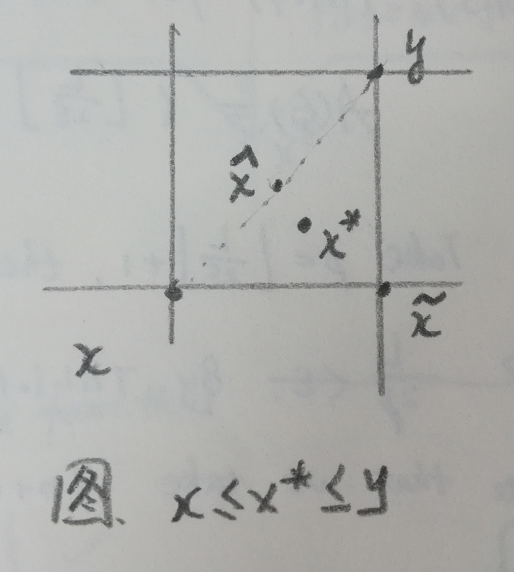
\includegraphics[width=0.3\textwidth]{figure/fig_1_theorem_1_1_1.png}
  \end{flushright}
  %%%



记:
\begin{equation*}
    \hat{x}  = (x+y)/2.
\end{equation*}
%Let us form a point $\tilde{x}^{}$ as follows
考虑网络点:
\begin{equation*}
    \tilde{x}^{(i)} = \left\{
     \begin{array}{cl}
        y^{(i)}, & \textnormal{if } x^{*(i)} \geq \hat{x}^{(i)} \\
        x^{(i)}, & \textnormal{otherwise }  \\
     \end{array}\right.
\end{equation*}
显然:
\begin{equation*}
        |\tilde{x}^{(i)} - x^{*(i)} | \leq \frac{1}{2p}.
\end{equation*}
$\Rightarrow$ $\|\tilde{x}-x^*\|_{\infty}^{}  = \max_{i}^{} |\tilde{x}^{(i)} - x^{*(i)} | \leq \frac{1}{2p}$.
  $\tilde{x}$ 属于网格之中
$\Rrightarrow$
\begin{equation*}
    f(\bar{x}) - f(x^*) \leq f(\tilde{x}) - f(x^*) \leq L \|\tilde{x}-x^*\|_{\infty}^{} \leq \frac{L}{2p}.
\end{equation*}

%\myendproof

%proof end.
{\mbox{} \hfill{\small
\textrm{$\Box$}}\vspace{1ex}}



% \framebreak

% \begin{itemize}
% \item  找到属于网格中的 $\tilde{x}$ , 其中 $\tilde{x}$ 位于 $x^*$附近:   $|\tilde{x}^{(i)} - x^{*(i)} | \leq \frac{1}{2p}$.
% \item  利用 $f$的Lipschitz 假设: 如果 $\tilde{x}$ 位于$x^*$附近 $\Rightarrow$
%     $f(\tilde{x})$ 也在 $f(x^*)$附近.

% \item \blue{
% * $f$的Lipschitz假设意味着$f$的变化率受常数$L$的约束 :
%   \begin{equation*}
%     \frac{f(x)-f(y)}{\|x-y\|} \leq L.
%   \end{equation*}
% } % end red

% \end{itemize}

\framebreak

\textbf{ 分析复杂度.}

%让我们完成问题类的定义。
定义目标如下:
\begin{equation}\label{EQ_stop_rule_epsilon}
    \textnormal{找到 }\ \bar{x} \in B_n: \ f(\bar{x}) -  f^* \leq \epsilon.
\end{equation}

\begin{corollary}
    方法 $\mathcal{G}$的问题(\ref{EQ_box_constrain_f}), (\ref{EQ_f_Lipschitz}) 和  (\ref{EQ_stop_rule_epsilon})的分析复杂度:
     最多为
    \begin{equation*}
        \mathcal{A}(\mathcal{G}) = \left( \bigg{\lfloor}\frac{L}{2\epsilon}\bigg{\rfloor}  +2 \right)^{n}
    \end{equation*}
\end{corollary}


\begin{proof}
    令 $p=\left( \big{\lfloor}\frac{L}{2\epsilon} \big{\rfloor}  +1\right)$, 则 $p> \frac{L}{2\epsilon}$.
    由定理 \ref{TH_complexity_uniform_grid}知, $f(\bar{x}) - f^* \leq \frac{L}{2p} < \epsilon$. \\
    \footnotehint{注.我们构造了 $(p+1)^n$ 个点.}
\end{proof}

\framebreak

\textbf{注.}

\begin{itemize}
    \item \blue{$\mathcal{A}(\mathcal{G})$ 给出了问题类的复杂度上限} 

    \item 问题 1. 我们的证明可能过于粗略, $\mathcal{G}(p)$ 的实际性能要好得多.

    \item 问题 2. 我们仍然不能确定 $\mathcal{G}(p)$ 是求解问题 (\ref{EQ_box_constrain_f})的合理方法. 可能存在其他性能高得多的方案.
\end{itemize}

\end{frame}

\begin{frame}[allowframebreaks]
\frametitle{复杂度下限}
% \textbf{复杂度下限}


需要给出问题(\ref{EQ_box_constrain_f}), (\ref{EQ_f_Lipschitz}) 和  (\ref{EQ_stop_rule_epsilon})的复杂度下界.
主要特征: 

 \begin{itemize}
\item  \blue{基于黑盒概念} 
\item \blue{这些边界对于所有合理的迭代方案都是有效的 }   $\rightarrow$提供了
\blue{问题类的分析复杂度的下限} 
\item 这种下界 通常 基于\blue{对抗 oracle}的思想  
\end{itemize}


\framebreak

\textbf{对抗oracle的概念}

\begin{itemize}
\item 对抗oracle: \blue{为每种具体方法创建一个最坏的问题} 
\item  它从一个“空”函数开始, \hint{ “以最坏的方式” 回应算法的每次提问}
%{it tries to answer each call of the method in the worst possible way}.
\item  答案必须 \blue{与之前的答案和问题类别的描述相一致}
%\item 请注意,在方法终止后\blue{可以重建问题}, 这完全符合该方法的最终信息集.
%\item  如果在这个问题上使用这个方法, 它将重现相同的测试点序列
%,因为它将从oracle得到相同的答案.
\end{itemize}

\framebreak

考虑对抗Oracle是如何解决这个问题 (\ref{EQ_box_constrain_f})的. 考虑问题 $\mathcal{C}$:
\bigskip

\begin{center}
	 
\begin{tabular}{|l|l|}
\hline
\multirow{2}{*}{\textbf{模型}} &  $\min_{x\in B_n}^{} \ f(x) $ \\
            &  $f(x)$ 是在 $B_n$上 $l_\infty$-Lipschitz 连续的 . \\[2ex]
\hline
 \textbf{Oracle}  &  零阶局部黑盒. \\[2ex]
 \hline
\textbf{近似解}&  找到 $\bar{x}\in B_n : f(\bar{x})-f^* \leq \epsilon$. \\[2ex]
\hline
\end{tabular}

\end{center}


\framebreak

\begin{theorem}\label{TH_lower_bound_uniform_grid}(复杂度下限)
  对于 $\epsilon<\frac{L}{2}$,  对于零阶方法,$\mathcal{C}$的分析复杂度至少为 
   $\left( \big{\lfloor}\frac{L}{2\epsilon} \big{\rfloor} \right)_{}^n$.
\end{theorem}




\begin{proof}
%\textbf{Proof.}

记 $p = \left( \big{\lfloor}\frac{L}{2\epsilon} \big{\rfloor} \right) \geq 1$.
假设存在一种方法需要$N<p^n$ 次调用 oracle 来解决问题类 $\mathcal{C}$.
将算法应用于如下的对抗策略中:

\myfbox{0.7\textwidth}{
    在每一个测试点$x$处,Oracle 返回 $f(x) = 0$ .
}
这个方法找到的解 $\bar{x} \in B_n$ 满足 $f(\bar{x}) = 0$.
然而, 我们注意到存在$\hat{x} \in B_n$, 满足
\begin{equation*}
    \hat{x} + \frac{1}{p} \mathbf{1} \in B_n, \quad \mathbf{1} = (1,1,\ldots,1)_{}^T \in R^n
\end{equation*}
并且集合中没有测试点:
\begin{equation*}
    B = \{x\,|\,  \hat{x} \leq x \leq \hat{x}+ \frac{1}{p} \mathbf{1} \}
\end{equation*}

记
\begin{equation*}
    x^* = \hat{x} + \frac{1}{2p} \mathbf{1}.
\end{equation*}
考虑函数:
\begin{equation*}
    f(x) = \min\{0,L\|x-x^* \|_{\infty}^{} - \epsilon \}.
\end{equation*}

  \begin{center}
  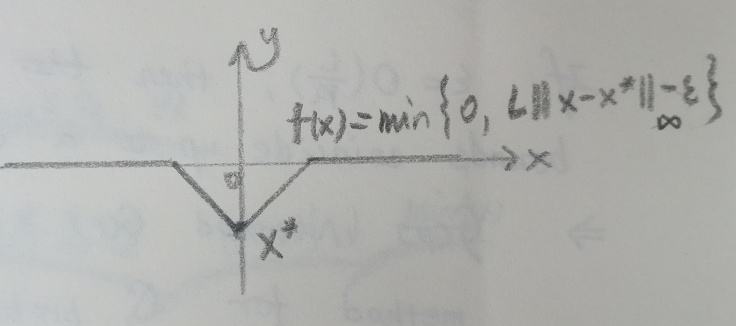
\includegraphics[width=0.6\textwidth]{figure/fig_1_theorem_1_1_2.png}
  \end{center}
  %%%
显然, $f(x)$ 是 $L_\infty$-Lipschitz 连续函数, 常数为$L$, 其全局最优值为 $-\varepsilon$.

% \mynote{
   $ \forall x_1,x_2 \in B$, $|f(x_1)-f(x_2)| \leq | L\|x_1-x^*\|_{\infty}^{} - L\|x_2-x^*\|_{\infty}^{}  | \leq L\|x_1-x_2\|_{\infty}^{}$.
% }

此外, $f(x)$ 只有在集合中不为0
\begin{equation*}
    B' = \{x\,|\, \|x-x^*\|_{\infty}^{}\leq \frac{\epsilon}{L}\}
\end{equation*}
由$2p \leq \frac{L}{\epsilon}$得:
\begin{equation*}
    B' \subseteq B = \{x\,|\, \|x-x^*\|_{\infty}^{} \leq \frac{1}{2p}\}.
\end{equation*}

%%%
  \begin{flushright}
  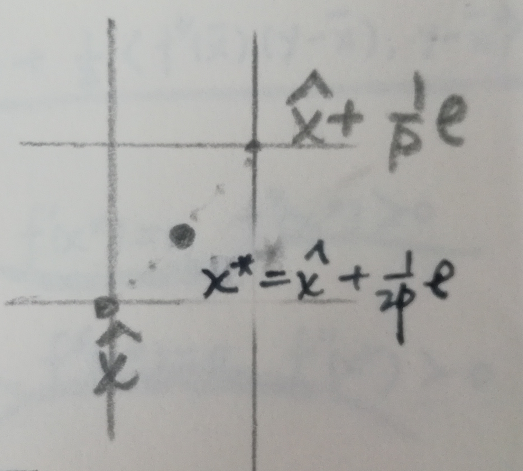
\includegraphics[width=0.3\textwidth]{figure/fig_2_theorem_1_1_2.png}
  \end{flushright}

因此,
\begin{itemize}
    \item $f(x)$ 在所有测试点处都等于0.
    \item 这个方法所得结果的精度为$\epsilon$.
\end{itemize}

故有如下结论: 如果调用 oracle 的次数小于 $p^n$, 结果的精确度不会优于 $\epsilon$.

\end{proof}
\end{frame}


\begin{frame}
\frametitle{均匀网格法复杂度}
\
\textbf{$\mathcal{G}(p)$ 是问题类$\mathcal{C}$}的一个 \dred{最优方法}
\bigskip

现在我们可以对均匀网格方法的性能做更多的介绍。
将均匀网格法复杂度的上界与下界进行比较:

\bigskip
\begin{tabular}{ll}
 上界& $ \left( \big{\lfloor}\frac{L}{2\epsilon} \big{\rfloor} +2 \right)_{}^n$ \\
 下界 & $ \left( \big{\lfloor}\frac{L}{2\epsilon} \big{\rfloor} \right)_{}^n$ \\
\end{tabular}

\bigskip

因此, 如果 $\epsilon = O(\frac{L}{n})$, \blue{则下界和上界相同,仅差一个常值乘数因子.}
这表明均匀网格法 $\mathcal{G}(p)$ 是问题类 $\mathcal{C}$的一个最优方法.


\end{frame}



\begin{frame}
\frametitle{一般的优化问题是不可解的}

%At the same time,
 \dred{定理 1.1.2 支持我们最初的说法,即一般优化问题是不可解决的.}
%Let us look at the following example.

\begin{example}
例题 1.1.4 考虑由以下参数定义的问题类 $\mathcal{F}$ :
\begin{equation*}
    L = 2;\quad n = 10;\quad \epsilon = 0.01
\end{equation*}
%Note that
%the size of the problem is very small and we ask only for 1\% accuracy.
 \blue{  此问题类的复杂度下限是
$ \left( \frac{L}{2\epsilon}  \right)_{}^n$.}
%Let us compute what this means.

\begin{tabular}{ll}
复杂度下界: &  $10_{}^{20}$ 次oracle调用 \\
单次 Oracle 调用的计算复杂度: & 至少$n$ 次算术运算 \\
总复杂度: & $10_{}^{21}$ 算术运算 \\
计算机运算速度: & $10^6$ 算术运算/秒 \\
总时间: & $10^{15}$秒 \\
一年: & 不到 $3.2 \times 10^7$ 秒. \\
我们需要: & 32 000 000 年. \\
\end{tabular}


\end{example}

\end{frame}




%==========================

\section{优化算法构造思想}

\begin{frame}[allowframebreaks]

\frametitle{松弛和近似}

广义非线性规划的\textbf{主要任务} : \dred{找到可微函数的局部极小值}.

%%%
  \begin{flushright}
  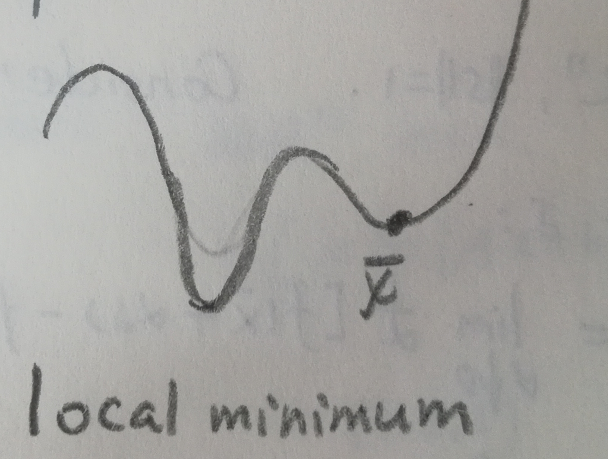
\includegraphics[width=0.3\textwidth]{figure/fig_1_sec1_2_1.png}
  \end{flushright}
  %%%


大多数非线性规划方法都是基于松弛的思想:

\myfbox{0.7\textwidth}{
我们称序列 $\{a_k^{}\}_{k=0}^{\infty}$  为一个 \textit{松弛序列}
 如果 $a_{k+1}^{}\leq  a_k,\quad \forall\, k\geq 0$.
}

\framebreak


考虑无约束最小化问题
\begin{equation}\label{EQ_min_f_unconstrain}
\min_{x\in R^n}^{}\ f(x),
\end{equation}
其中 $f$ 是一个光滑的函数.

我们生成一个松弛序列 $\{f(x_k) \}_{k=0}^{\infty}$:
\begin{equation*}
f(x_{k+1}) \leq f(x_k), \quad k=0,1,\ldots
\end{equation*}

这个方法有以下 \blue{重要优势}:

\begin{enumerate}
\item \blue{如果$f(x)$在$R_n$中有下界, 则序列 $\{f(x_k) \}_{k=0}^{\infty}$ 收敛.}
\item 在任何情况下,目标函数的初始值总能得到改进.
\end{enumerate}

\framebreak

松弛思想要付诸实施,离不开另一个优化的基本原则:
\dred{ 近似.}
%In general,

\myfbox{0.7\textwidth}{\dred{近似} 意味着用一个简化的函数代替复杂的函数,足够接近原始函数.
}

\end{frame}


%==========================
\section{梯度下降法}

\begin{frame}[allowframebreaks]


\frametitle{梯度的两个重要性质.}

用 $\mathcal{L}_f(\alpha)$ 表示\blue{ $f(x)$的水平集}:
$$
    \mathcal{L}_f(\alpha) = \{ x\in R^n \,|\, f(x)\leq \alpha \}.
$$
考虑\blue{在 $\bar{x}$处与 $\mathcal{L}_f(f(\bar{x}))$相切的方向集 :}
$$
    S_f(\bar{x}) = \left\{ s\in R^n \,|\,  s= \lim_{y_k\rightarrow \bar{x}, f(y_k)=f(\bar{x}) }^{}  \frac{y_k-\bar{x}}{\|y_k-\bar{x}\|} \right\}.
$$

\textbf{性质1.  梯度矢量垂直于水平集的“切线方向”.}

\begin{lemma}\label{lemma_1_2_1}

    如果$s\in S_f(\bar{x})$, 那么$\langle f'(\bar{x}), s\rangle =0$.

\end{lemma}

\begin{proof}
    由于
    $$
        f(y_k) = f(\bar{x}) + \langle f'(\bar{x}),y_k-\bar{x} \rangle + o(\|y_k-\bar{x}\|) = f(\bar{x}).
    $$
    因此, $\langle f'(\bar{x}),y_k-\bar{x} \rangle + o(\|y_k-\bar{x}\|) = 0$.
    将该方程除以$\|y_k-\bar{x}\|$ 并取$y_k \rightarrow \bar{x}$中的极限, 得到结果.
\end{proof}


\framebreak

\textbf{性质2. 负梯度 $-f'(\bar{x})$ 是$f(x)$在点 $\bar{x}$处局部下降最快的方向 .
}

\begin{proof} 
设 $s$ 为 $R^n$中的一个方向 , $\|s\| = 1$.
\blue{考虑 $f(x)$ 沿 $s$的局部递减:}
$$
    \Delta(s) = \lim_{\alpha \downarrow 0}^{} \frac{1}{\alpha} [f(\bar{x}+\alpha s) - f(\bar{x})].
$$
注意 $f(\bar{x}+\alpha s) - f(\bar{x}) = \alpha \langle f'(\bar{x}),s\rangle + o(\alpha)$.
因此
$$
    \Delta(s) = \langle f'(\bar{x}), s\rangle.
$$
利用 Cauchy-Schwartz不等式:
$$
    -\|x\| \cdot \|y\| \leq \langle x,y\rangle \leq \|x\|\cdot \|y\|,
$$
得到: $\Delta(s) = \langle f'(\bar{x}), s \rangle \geq -\|f'(\bar{x})\|$. 令
$ 
    \bar{s} = - f'(\bar{x})/\|f'(\bar{x})\|.
$ 
$\Rightarrow$
$ 
    \Delta(\bar{s}) = - \langle f'(\bar{x}), f'(\bar{x}) \rangle / \|f'(\bar{x})\| = - \|f'(\bar{x}\|.
$ 
\hint{ $\Rightarrow$方向 $-f'(\bar{x})$ (负梯度) 是$f(x)$ 在点$\bar{x}$ 处局部下降最快的方向.
} 
\end{proof}

\end{frame}


\begin{frame}[allowframebreaks]


\frametitle{梯度下降法} 

\blue{我们已经知道负梯度方向是可微函数局部下降最快的方向.}
由于我们要找到这种函数的 \blue{局部极小值} , 下面是尝试的第一个方法:


\myfbox{0.7\textwidth}{
\begin{center}
    \textbf{梯度法}
\end{center}

\textbf{选择 } $x_0\in R^n$.

\textbf{迭代} $x_{k+1}^{} = x_{k} - h_k f'(x_k)$, $k=0,1,\ldots$.
}

%我们将把这个方案称为 \blue{梯度法.}
 $h_k>0$:  \blue{步长}.
%Of course, it must be positive.

%There are many variants of this method, which differ one from another by the \blue{step-size
%strategy.}
 %Let us consider the most important examples.
\end{frame}


\begin{frame}[allowframebreaks]
\frametitle{重要的步长策略.}

\begin{enumerate}
\item 序列 $\{h_k\}_{k=0}^{\infty}$ 是 \blue{提前选定的.}例如,
$$
    \begin{aligned}
        h_k & = h >0, \qquad \textnormal{(恒定步长)} \\
        h_k & = \frac{h}{\sqrt{k+1}}. \\
    \end{aligned}
$$

\item \blue{完全松弛.}
$$
    h_k = \textnormal{argmin}_{h\geq 0} \ f(x_k-hf'(x_k)).
$$

\item \blue{Goldstein-Armijo准则:} 寻找$x_{k+1}^{} = x_{k}^{} - h f'(x_k)$ 满足
\begin{align}
    f(x_k) - f(x_{k+1}) & \geq \alpha \langle f'(x_k), x_k - x_{k+1}^{} \rangle \label{EQ_1_2_10} \\
        f(x_k) - f(x_{k+1}) & \leq \beta \langle f'(x_k), x_k - x_{k+1}^{} \rangle  \label{EQ_1_2_11}
\end{align}
其中$0<\alpha < \beta < 1$ 是固定参数.

\end{enumerate}

\framebreak
\textbf{注意}
\begin{itemize}
\item 第一种策略 (i.e, \blue{提前选定})是最简单的. 它是实际应用中,特别是凸优化情况下最常见的方法 .


\item 第二种策略 (i.e., \blue{完全松弛}) 是理论上的方法.


\item 第三种策略 (i.e., \blue{Goldstein-Armijo准则}) 在许多非线性规划算法中广泛使用.

\framebreak

\textbf{Goldstein-Armijo准则的几何解释}

固定 $x\in R^n$. 考虑关于变量的一元函数
$$
    \phi(h)  = f(x-h f'(x)), \quad h\geq 0.
$$
则该策略可接受的步长值位于两个线性函数之间:
$$
\begin{aligned}
    \phi_1(h) & = f(x) - \alpha h \|f'(x)\|^2, \\
    \phi_2(h) & = f(x) - \beta h \|f'(x)\|^2. \\
\end{aligned}
$$
其中 $\phi(0) = \phi_1(0) = \phi_2(0)$ 且 $\phi'(0) < \phi_2^{\prime}(0) < \phi_{1}^{\prime}(0) < 0$.

因此, 只要 $\phi(h)$ 的下界存在,可接受的值一定存在.
\end{itemize}
\framebreak

% \mynote{
\begin{itemize}
\item    如果我们表示为:
    $$
    \begin{aligned}
         \phi(h) & = f(x^k + h d^k) - f(x^k),\\
         \phi_1(h) &= \beta \nabla f(x^k)^T d^k \cdot h \\
         \phi_2(h) &= \alpha \nabla f(x^k)^T d^k \cdot h, \\
    \end{aligned}
    $$
    那么 Goldstein-Armijo 准则可以重新定义为
    $$
        \phi_1(h)  \leq \phi(h) \leq \phi_2(h).
    $$
 \item 不等式 (\ref{EQ_1_2_11}) $   f(x_k) - f(x_{k+1})  \leq \beta \langle f'(x_k), x_k - x_{k+1}^{} \rangle$
    意味着步长$h$应该有一个下界.
 \end{itemize}
% }

\end{frame}


\begin{frame}
  \frametitle{几何递减的步长不合理}

\begin{itemize}
  \item 几何递减步长 (提前选定的)
  $$
  h_k = h\cdot \omega^k,\qquad \omega\in (0,1).
  $$
例如 $h_k = 0.5^k$, $k=0,1,\cdots$.

\end{itemize}

\begin{itemize}
\item $h_k = 0.5^k$, $k=0,1,\cdots$ $\Rightarrow$
  $\sum_{k=0}^{\infty} 0.5^k = 2$

\item  $\Rightarrow$ 可能的搜索区域有限: $\{x_k\} \subseteq   \mathbf{B}(x_0, 2)$

\item   $\Rightarrow$ 无法到达 $x^*$ 如果 $\|x^* - x_0 \|\geq 2$.

\end{itemize}
\end{frame}


\begin{frame}[allowframebreaks]


  \frametitle{评估梯度法的性能(讲解)}

考虑问题
$$
    \min_{x\in R^n} \ f(x),
$$
其中\blue{$f\in C_{L}^{1,1}(R^n)$.
假定 $f(x)$ 在 $R^n$上有下界.}


\bigskip
\textbf{评估一个梯度步长的目标函数的下降量}

\bigskip

考虑 $y = x- h f'(x)$. 则有
\begin{equation}\label{EQ_1_2_12}
\begin{aligned}
    f(y) & \leq f(x) + \langle f'(x), y-x \rangle + \frac{L}{2} \|y-x\|^2 \\
        &  = f(x) -h \| f'(x)\| + \frac{h^2}{2} L \|f'(x)\|^2 \\
        &  = f(x) - h(1-\frac{h}{2}L) \|f'(x)\|^2. \\
\end{aligned}
\end{equation}

\framebreak

为了获得目标函数下降量的最佳估计:
$$
    \Delta(h) = -h(1-\frac{h}{2}L) \longrightarrow \min_{h}^{}.
$$

计算此函数的导数 $\longrightarrow$
最佳步长必须满足以下方程:
$$
    \Delta'(h) = hL - 1 =0.
$$
因此,  在 $\Delta''(h) = L>0$的情况下,可以得到$\Delta(h)$的最优解为 $h^* = \frac{1}{L}$ .

因此, 我们证明了梯度下降法一次迭代后目标函数值的下降量:
$$
   \blue{ f(y) \leq f(x) - \frac{1}{2L} \|f'(x)\|^2. }
$$

\framebreak

\blue{注.} 
\begin{itemize}
	\item 
迭代格式:
 $y = x - h f'(x)$.

\item 
对 $f\in C_{L}^{1,1} R^n$, 一次迭代后的目标函数下降量 \dred{至少为}
 $h(1-\frac{h}{2}L) \|f'(x)\|^2 $ %由式(\ref{EQ_1_2_12})得.

\item 
 令 $h = 1/L$ $\rightarrow$ $\rightarrow$
   一次迭代 目标函数值下降量的最佳估计:
 $\frac{1}{2L} \|f'(x)\|^2$ 

\end{itemize}

\framebreak

\bigskip
\textbf{考虑具体的步长策略:}
\bigskip

设 \blue{$x_{k+1}^{} = x_{k} - h_k f'(x_k)$}

\begin{enumerate}
\item 对于恒定步长策略 $h_k \equiv h$:
$$
    f(x_k) - f(x_{k+1}^{}) \geq   h_k (1-\frac{h_k}{2}L) \|f'(x_k)\|^2.
$$
 最优步长选择: $h_k = 1/L$.

\item 对完全松弛策略,有
$$
    f(x_k) - f(x_{k+1}^{}) \geq   \frac{1}{2L} \|f'(x_k)\|^2
$$
\footnotehint{ 上面的单步下降量 并不比 $h_k = \frac{1}{L}$的下降量更大 
}


\item  基于Goldstein-Armijo 准则 (\ref{EQ_1_2_11}): 
$$
    f(x_k) - f(x_{k+1}^{}) \leq   \beta \langle f'(x_k),x_k-x_{k+1} \rangle  = \beta h_{k}^{} \|f'(x_k)\|^2
$$
由公式(\ref{EQ_1_2_12}) \footnotehint{$f(y)\leq f(x) - h(1-\frac{2}{Lh}) \|f'(x)\|^2$:}
$$
    f(x_k) - f(x_{k+1}^{}) \geq    h_{k}^{}(1-\frac{h_k}{2} L) \|f'(x_k)\|^2.
$$
$\Rightarrow$ $h_k \geq \frac{2}{L} (1-\beta)$
利用公式(\ref{EQ_1_2_10}) \footnotehint{$f(x_k) - f(x_{k+1} ) \geq \alpha \langle f'(x_k), x_{k}-x_{k+1}\rangle$}: 
$$
    f(x_k) - f(x_{k+1}^{}) \geq \alpha \langle f'(x_k),x_k-x_{k+1} \rangle  = \alpha h_k \|f'(x_k)\|^2.
$$
与前面的不等式结合  $\rightarrow$
$$
  f(x_k) - f(x_{k+1}^{}) \geq  \frac{2}{L} \alpha (1-\beta)  \|f'(x_k)\|^2.
$$

\footnotehint{$\rightarrow$基于各种步长规则($w>0$):  
\begin{equation}\label{EQ_1_2_13}
    f(x_k) - f(x_{k+1}^{}) \geq \frac{w}{L} \|f'(x_k)\|^2.
\end{equation} 
}
\end{enumerate}

\mynote{
 $\bullet$ $f\in C_L^{1,1}(R^n)$

 $\bullet$ 不等式 (\ref{EQ_1_2_11}): $   f(x_k) - f(x_{k+1})  \leq \beta \langle f'(x_k), x_k - x_{k+1}^{} \rangle$

 $\Rightarrow$ 步长 $h$ 有下界 $h_k\geq {2}{L}(1-\beta)$.
}

\end{frame}


\begin{frame}[allowframebreaks]

\frametitle{评估梯度法的性能.}

将不等式 (\ref{EQ_1_2_13}):$ f(x_k) - f(x_{k+1}^{}) \geq \frac{w}{L} \|f'(x_k)\|^2.$ 关于 $k=0,\ldots,N$进行累加:
\begin{equation}\label{EQ_1_2_14}
    \frac{w}{L} \sum_{k=0}^N \|f'(x_k)\|^2 \leq f(x_0) - f(x_{N+1}^{}) \leq f(x_0) - f^*,
\end{equation}
其中 $f^*$ 是问题(1.2.1)的最优值  
$\Rightarrow$
$$
    \|f'(x_k)\| \rightarrow 0,  \textnormal{\quad 当 \quad} k\rightarrow \infty.
$$

 

\textbf{收敛速度}

记
$
    g_N^{*} = \min_{0\leq k\leq N}^{} g_k,
$
其中 $g_k = \|f'(x_k)\|$ 
$\Rightarrow$
\begin{equation}\label{EQ_1_2_15}
    g_N^{*} \leq \blue{\frac{1}{\sqrt{N+1}} }  \left[ \frac{L}{w} (f(x_0)-f^*) \right]_{}^{1/2}.
\end{equation}
\footnotehint{
不等式右边描述了序列$\{g_N^*\}$收敛到0的速度.
\dred{但是,这并不是序列 $\{f(x_k)\}$ 和 $\{ x_k\}$的收敛速度.}
}
\end{frame}


\begin{frame}[allowframebreaks]
\frametitle{梯度法只能找到一个稳定点(讲解)}

 在一般的非线性优化中,我们的目标是相当宽松的:
我们想要 \blue{找到问题的局部极小值}.
\dred{  然而, 即使是这个目标梯度方法也是无法实现的.}
%Let us consider the following example.


\begin{example}\label{example_1_2_2}
    考虑二元函数:
    $$
        f(x) = f(x_1,x_2) = \frac{1}{2}x_1^2 + \frac{1}{4} x_2^4 - \frac{1}{2} x_2^2.
    $$
   该函数的梯度为:
    $$
        f'(x) = (x_1,x_2^3 - x_2)_{}^{T}.
     $$
    因此,该函数的局部极小解之优可能在下述的三个点中取到:
    $$
        (0,0), \quad (0,-1), \quad (0,1).
    $$
\end{example}
\framebreak
\text{计算该函数的Hessian矩阵}
    $$
        f''(x) = \left[\begin{array}{cc}
                    1 & 0 \\
                    0 & 3x_2^2 -1 \\
                     \end{array}\right]
    $$


\begin{itemize}
\item   点$(0,1)$ 和点$(0,-1)$ 是孤立的局部极小值
%\footnote{事实上,在我们的例子中,它们是全局最优解}, 
但是 $x_1^*=(0,0)$ 只是我们函数的一个驻点.
   \item 对于充分小的 $\epsilon$,有$f(x_1^*) = 0$ 和 $f(x_1^* + \epsilon e_2) = \frac{\epsilon^4}{4} - \frac{\epsilon^2}{2}<0$  .

    \item 考虑梯度下降法自 $x_0 = (1,0)$开始的迭代点列的轨迹.
    注意这个点的第二个坐标是零。所以 $f'(x_0)$的第二个坐标也是零.
   \item 同样, $x_1$ 的第二个坐标也是零…
    $\rightarrow$ 由梯度下降法生成的迭代序列中的点第二个坐标都是0 
     $\rightarrow$  这个序列收敛于$x_1^*=(0,0)$
\end{itemize}
  %  To conclude our example, note that this situation is typical for all first-order unconstrained minimization methods.
  %  Without additional rather strict assumptions it is impossible to guarantee their global convergence
  %  to a local minimum, only to a stationary point.

\end{frame}



\begin{frame}[allowframebreaks]
\frametitle{复杂度上限}

\begin{itemize}
 \item 不等式 (\ref{EQ_1_2_15}) 提供了  
极小化序列的\blue{收敛速度}.

\item 收敛速度提供了问题类的复杂度的上界
%,这些上界已经被数值方法证明是合理的。

\item 如果存在一种算法,它的复杂度上界与问题类的复杂度下界成正比,称这种方法为\blue{最优方法}.

\end{itemize}


\framebreak

% 一个复杂度上界的例子.

\begin{example}\label{eg_1_2_3}

    考虑以下问题类:

    \begin{tabular}{|l|l|}
    \hline
    \textbf{模型} &   1. 无约束最小化. \\
        & 2.  $f\in C_{L}^{1,1}(R^n)$ \\
        & 3. $f(x)$ 是下界.   \\ \hline
   \textbf{Oracle} &
               一阶黑盒. \\ \hline
    \textbf{$\epsilon$-近似解} & $f(\bar{x}) \leq f(x_0)$, $\|f'(\bar{x}) \| \leq \epsilon$ \\ \hline
    \end{tabular}

\framebreak

%注意, 
不等式 (\ref{EQ_1_2_15})  $\Rightarrow$

$$
    g_{N}^{*} \leq \frac{1}{\sqrt{N+1}} \left[\frac{1}{w} L(f(x_0)-f^*) \right]_{}^{1/2}\leq \epsilon.
$$
  如果 $N+1 \geq \frac{L}{w\epsilon^2}(f(x_0)-f^*)$ $\Rightarrow$ $g_{N}^{*} \leq \epsilon$.

$\Rightarrow$ 该问题类 复杂度上限  \hint{$\frac{L}{w\epsilon^2}(f(x_0)-f^*)$ } 
\begin{itemize}
\item 对比定理1.1.2的结果 $\rightarrow$它的效果更好 
%至少它不依赖于 $n$.
\item \blue{这个问题类的复杂度下限是未知的.}
\end{itemize}
\end{example}


\end{frame}

\begin{frame}[allowframebreaks]
\frametitle{ 梯度法的局部收敛性}


考虑无约束最小化问题
$$
    \min_{x\in R^n} \ f(x)
$$
 假设:
\begin{enumerate}
    \item $f\in C_M^{2,2}(R^n)$.
    \item 存在函数$f$的局部极小值,在该极小值处Hessian矩阵是正定的.
    \item 我们知道:Hessian矩阵在最优解 $x^*$处有界:
    \begin{equation}\label{EQ_1_2_17}
        l I_n \preceq f''(x^*) \preceq L I_n.
    \end{equation}
    \item \blue{起始点 $x_0$ 充分靠近$x^*$.}
\end{enumerate}

\framebreak

考虑过程:
$$
    x_{k+1}^{} = x_k - h_k f'(x_k).
$$
注意 $f'(x^*) = 0$. 因此,
$$
\begin{aligned}
    f'(x_k)    & =f'(x_k) - f'(x^*) = \int_{0}^{1} f''(x^* + \tau(x_k-x^*)) (x_k-x^*) d\tau \\
        & =G_k (x_k-x^*) \\
\end{aligned}
$$
其中 $G_k = \int_0^1 f''(x^* + \tau(x_k-x^*)) d\tau$. 因此,
$$
    x_{k+1}^{} - x^* = x_k - x^* - h_{k}^{}G_k^{}(x_k-x^*) = (I-h_kG_k) (x_k-x^*).
$$

\framebreak


\begin{theorem}\label{TH_1_2_4}
    设函数$f(x)$ 满足我们的假设且初始点 $x_0$ 足够接近局部极小值:
    $$
        r_0 = \|x_0 - x^* \| < \bar{r} = \frac{2l}{M}.
    $$
    那么按式选取步长$h_k = \frac{2}{L+l}$的梯度下降法满足:
    $$
    \|x_k - x^*\| \leq \frac{\bar{r}r_0}{\bar{r}-r_0} \left(1-\frac{2l}{L+3l} \right)^k.
    $$
    \dred{这种收敛速度称为线性收敛速度.}
\end{theorem}


\framebreak

% \mynote{
\begin{itemize}
\item 收敛半径
        $$
            \bar{r} = \frac{2l}{M}
        $$
        与 $l$ 成比例,且与 $M$成反比, 其中
        \begin{enumerate}
        \item $l$ 是 $f''(x^*)$的最小特征值;
        \item $M$  是$f''(x)$的Lischitz常数.
        \end{enumerate}

\item 收敛速度取决于 $L$ 和 $l$ ,$f''(x^*)$的最大和最小的特征值.
在极端情况下 $L = l$ (注意 $L\geq l$),
      $$
    \|x_k - x^*\| \leq \frac{\bar{r}r_0}{\bar{r}-r_0}  (\frac{1}{2})^k.
    $$
然而, 当 $L>>l$时, 收敛明显较慢.比如 $L = 1000 l$, 则
      $$
    \|x_k - x^*\| \leq \frac{\bar{r}r_0}{\bar{r}-r_0}  (\frac{1001}{1003})^k.
    $$
注意 $(\frac{1001}{1003})^{300} \approx 0.55$, 这意味着与理想情况$L = l$ 相比,为了达到相同精度,在这种情况下迭代次数将是300次.
\end{itemize}
% }
\end{frame}





\begin{frame}[allowframebreaks]
\frametitle{总结}

\begin{itemize}
    \item[1.]\textbf{均匀网格法.} 在可行集内形成测试点的统一网格,
  并计算该网格上目标函数的最小值.

\begin{itemize}

\item    上界: $ \left( \big{\lfloor}\frac{L}{2\epsilon} \big{\rfloor} +2 \right)_{}^n$
\item  下界: $ \left( \big{\lfloor}\frac{L}{2\epsilon} \big{\rfloor} \right)_{}^n $


  \begin{itemize}
  \item[-] 均匀网格方法是一种\dred{优化方法} ,适用于解决: \\
     $\min_{x\in B_n}^{}\ f(x)$, 其中 $f$ 是 Lipschitz 连续的.
  \item[-] 一般的优化问题是不可解的.
  \end{itemize}

\end{itemize}

\item[2.] \textbf{松弛和近似.}一般非线性规划方法的构造主要基于两个手段

\begin{itemize}
    \item 松弛:如果 $\{a_k^{}\}_{k=0}^{\infty}$ 满足 
    $a_{k+1}^{}\leq  a_k,\quad \forall\, k\geq 0$
    则称其为\textit{松弛序列}
    \item 近似:用一个足够接近原始物体的简化物体来代替最初的复杂物体.
\end{itemize}

\end{itemize}

\end{frame}


\begin{frame}[allowframebreaks]

\begin{itemize}
    \item[3.] \textbf{梯度下降法.}
    $$x_{k+1} = x_k + h_k \cdot (-f'(x_k)), k=0,1,2,\cdots$$

\begin{itemize}

\item 步长策略:
\begin{enumerate}
\item 提前选定: $h_k \equiv h$; $h_k = \frac{h}{\sqrt{k+1}}$;
\item 完全松弛
\item Golstein-Armijo准则
\end{enumerate}

\item   梯度法的复杂性

  \begin{itemize}
    \item[-] 梯度下降法一次迭代后目标函数值的可能的下降量为:
     $$
        f(x_k) - f(x_{k+1}) \geq \frac{w}{L} \|f'(x_k)\|^2.
     $$

    \item[-] 梯度法的复杂度

     % $\Longrightarrow $ 
     $$\frac{w}{L} \sum_{k=0}^{N} \|f'(x_k)\|^2 \leq f(x_0) - f(x_{N+1}) \leq f(x_0) - f^* ,$$
     $$\rightarrow \lim_{k\rightarrow \infty}^{} \|f'(x_k)\| = 0$$
    \item[-] 收敛速度\\
     记 $g_N^{*} = \min_{0\leq k \leq N} \|f'(x_k)\|$, 则
      $$
        g_N^{*} \leq \frac{1}{\sqrt{N+1}} [\frac{L}{w} (f(x_0)-f^*)]_{}^{1/2}.
     $$

     \item[-] \hint{
$f\in C_{L}^{1,1}(R^n)$, $f$ 有下界, 梯度法复杂度上界:
        $$
        \frac{L}{w\epsilon^2}(f(x_0) - f^*)
        $$
     } 


  \end{itemize}

     \item 局部收敛: 线性收敛速度

     $$
    \min_{x\in R^n} \ f(x)
$$
在给定假设下, 按$h_k^{*} = \frac{2}{L+l}$ 选取步长的梯度下降法收敛如下:
$$
    \|x_k - x^* \| \leq \frac{\bar{r}r_0}{\bar{r}-r_0} \left(1-\frac{2l}{L+3l}\right)^{k}.
$$


\end{itemize}
 
\end{itemize}
\end{frame}




\begin{frame}
	\frametitle{作业题} 
	
	
	\begin{enumerate}
 
		\item 编程题:第1部分第1节中,有练习题: 自行选取二分类数据集,编程实现 梯度下降法 求解Logistic 回归模型,并对数据集进行分类,计算分类准确率。
		请 在此基础上,使用  Armijo 准则确定每一次迭代的步长: 
		
		
		
	 
	 \blue{ Armijo准则:} 寻找$x_{k+1}^{} = x_{k}^{} - h f'(x_k)$ 满足
		\begin{align}
			f(x_k) - f(x_{k+1}) & \geq \alpha \langle f'(x_k), x_k - x_{k+1}^{} \rangle \label{EQ_1_2_10} 
		\end{align}
		其中$0<\alpha  < 1$ 是固定参数.
		
		
		
		
		
		
		
	\end{enumerate}
	
	
\end{frame}

\end{document}

